\section{HARDWARE RESULTS}


\subsection{INDUCTION MOTOR}

Induction motors, also known as asynchronous motors, are widely used in various industrial applications due to their simplicity, durability, and cost-effectiveness. They operate on the principle of electromagnetic induction, wherein a rotating magnetic field in the stator induces a current in the rotor, thus creating torque.

\begin{figure}[H]
	\centering
	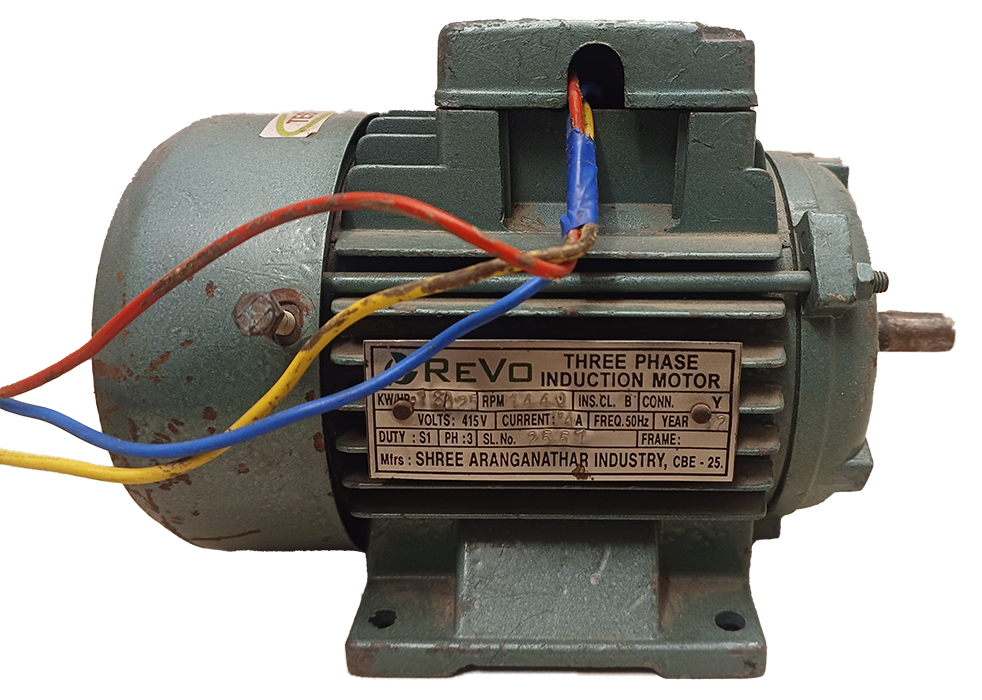
\includegraphics[width=4.0in]{sections/section4/images/inductionMotor/revo.png}
	\caption{Image of Induction Motor}
\end{figure}

We are utilizing a Revo 3-phase induction motor with the following specifications:

\begin{table}[H]
	\centering
	\begin{tabular}{|c|c|}
		\hline
		\textbf{Parameter} & \textbf{Value} \\ \hline
		Power & 0.25 Hp \\ \hline
		Voltage & 415 V (L-L) RMS \\ \hline
		Current & 1.4 A \\ \hline
		Frequency & 50 Hz \\ \hline
		Speed & 1440 rpm \\ \hline
		Phase & 3 \\ \hline
	\end{tabular}
	\caption{Nameplate Details of Induction motor}
\end{table}



\subsection{F28379D LAUNCHPAD}

The F28379D Launchpad, officially known as the LAUNCHXL-F28379D, is a powerful development board from Texas Instruments, designed around the TMS320F28379D microcontroller. This microcontroller is part of the C2000™ Piccolo™ family, renowned for its high-performance processing capabilities, which are particularly suited for engineering applications requiring real-time processing and control.

\textbf{Core Features:}
\begin{itemize}
    \item \textbf{Processor:} The TMS320F28379D microcontroller features a dual-core configuration with a C28x CPU and a secondary CLA (Control Law Accelerator) CPU, enhancing its ability to handle complex control algorithms.
    \item \textbf{Memory:} It includes onboard flash memory and RAM, facilitating robust applications and advanced computation.
    \item \textbf{Connectivity:} Provides extensive connectivity options including CAN, USB, and Ethernet, supporting a wide range of communication protocols.
    \item \textbf{Analog and Digital I/O:} Equipped with multiple ADC (Analog-to-Digital Converter) channels, DAC (Digital-to-Analog Converter) outputs, and PWM (Pulse Width Modulation) outputs for comprehensive sensor integration and actuator control.
\end{itemize}

\textbf{Applications:}
The F28379D Launchpad is particularly adept at handling applications that require real-time processing capabilities such as motor control, renewable energy systems, power supplies, and advanced sensing systems. Its high-speed processing and diverse I/O options make it ideal for both academic research and industrial applications.

\begin{figure}[H]
    \centering
    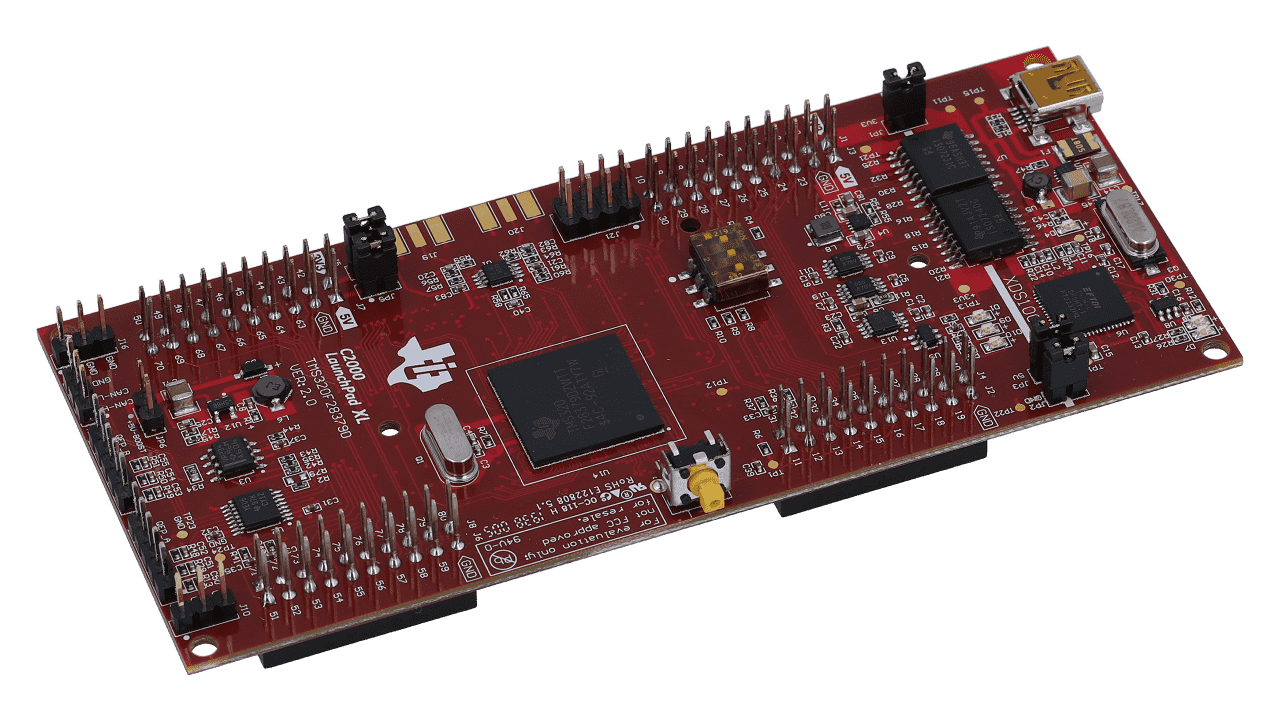
\includegraphics[width=4in]{sections/section4/images/f23879d/launchxl-f28379d-angled.png}
    \caption{Image of F28379D Launchpad}
\end{figure}

The integration of the F28379D Launchpad in projects offers a robust platform for developing sophisticated control systems and algorithms, facilitating innovation and efficiency in system design and implementation.



\subsection{INTELLIGENT POWER MODULE FSAM20SH60A}


We integrated the FSAM20SH60A, a Motion SPM\textsuperscript{\textregistered} 2 module, as a fundamental component. This device is UL Certified (No. E209204 UL1557) and serves as a high-performance 3-phase IGBT inverter with integrated gate drivers and protection, making it an ideal solution for AC Induction, BLDC, and PMSM motors.

\textbf{Key Features:}
\begin{itemize}
    \item \textbf{Efficiency and Safety:} Designed with low-loss, short-circuit rated IGBTs and an optimized gate drive to minimize electromagnetic interference (EMI) and losses. It incorporates multiple on-module protection features such as under-voltage lockouts, over-current shutdown, thermal monitoring, and fault reporting, ensuring robust and reliable operation.
    \item \textbf{Thermal Management:} Features low thermal resistance through the use of a ceramic substrate. It also includes separate open-emitter pins from low-side IGBTs for three-phase current sensing, supporting a wide variety of control algorithms.
    \item \textbf{Performance Specifications:} Tailored for a 15 kHz switching frequency with a built-in NTC thermistor for accurate temperature monitoring. It operates on a single-grounded power supply and offers an inverter power rating of 1.5 kW at an input voltage range of 100~253 VAC.
    \item \textbf{Customization and Isolation:} Provides an adjustable current protection level, allowing for customization via the selection of Sense-IGBT Emitter's external Rs. Boasts an impressive isolation rating of 2500 Vrms per minute.
    \item \textbf{High-Voltage Integrated Circuit:} The high-speed HVIC integrated into the FSAM20SH60A requires only a single supply voltage and effectively translates the incoming logic-level gate inputs to the high-voltage, high-current drive signals required to properly drive the module's internal IGBTs.
\end{itemize}

\begin{figure}[H]
    \centering
    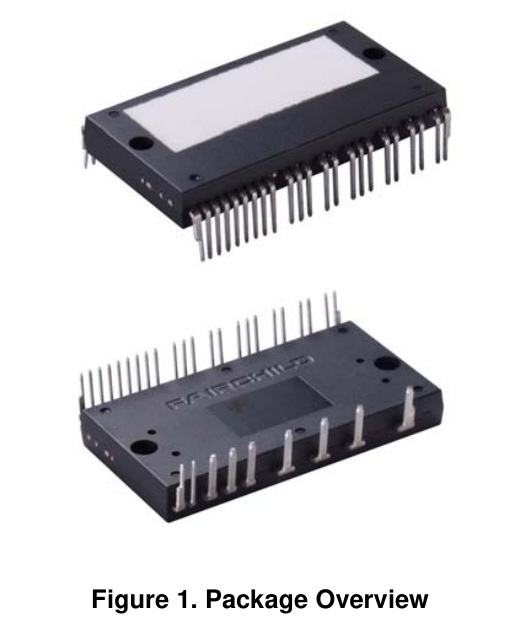
\includegraphics[width=3in]{sections/section4/images/IPM/ipm.png}
    \caption{Image of FSAM20SH60A module}
\end{figure}

This integration of the FSAM20SH60A enhances our project by providing a compact, efficient, and reliable solution for motor control applications, supporting our objectives of achieving high performance and durability in our designs.


\subsection{PCB DESIGN FOR FSAM20SH60A}

In the PCB design section of our project, we developed a printed circuit board for the FSAM20SH60A, an intelligent power module. Our design approach was heavily influenced by the application circuit provided in the module's datasheet.

\textbf{Design Considerations:}
\begin{itemize}
    \item \textbf{Reference Design:} The application circuit from the datasheet served as a crucial reference, ensuring adherence to the technical specifications and requirements of the FSAM20SH60A.
    \item \textbf{Component Placement and Trace Routing:} Special attention was given to the layout and routing of circuit traces and the strategic placement of components, focusing particularly on effective thermal management.
    \item \textbf{Functional Integration:} The design accommodates features such as three-phase current sensing and a single-grounded power supply setup. It also supports the functionality of the built-in NTC thermistor for temperature monitoring and the high-speed HVIC.
    \item \textbf{Customization Features:} Provisions were made for adjusting the current protection level through the selection of Sense-IGBT Emitter's external Rs.
\end{itemize}

\textbf{Tools Used:}
Software tools from National Instrument's circuit design suite were utilized. Multisim 14.3 aided in schematic capture, while Ultiboard 14.3 facilitated the PCB layout design.

\begin{figure}[H]
	\centering
	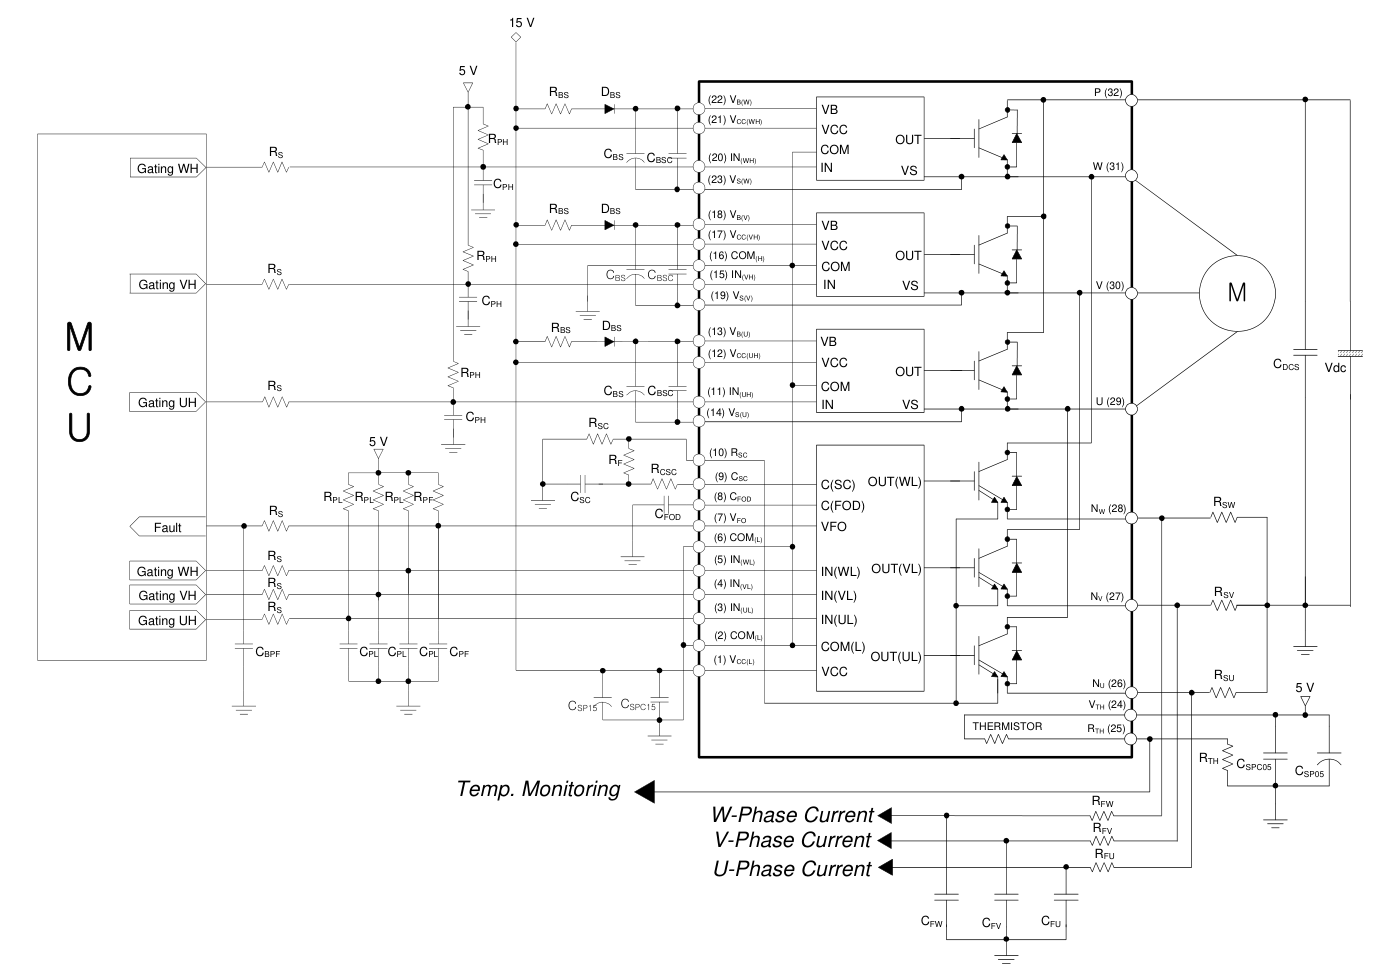
\includegraphics[width=6in]{sections/section4/images/PCBDesign/ApplicationCircuitfromDatasheet.png}
	\caption{Application Circuit from FSAM20SH60A Datasheet}
\end{figure}

\begin{figure}[H]
	\centering
	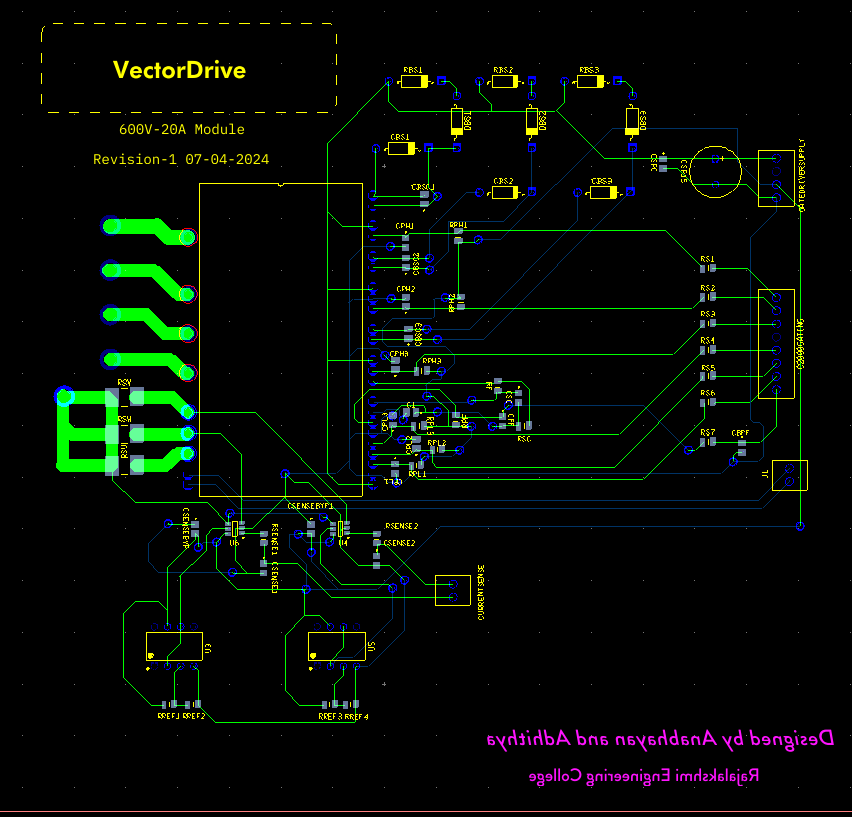
\includegraphics[width=4in]{sections/section4/images/PCBDesign/Ultiboard/Ultiboard.png}
	\caption{PCB Layout Design in Ultiboard}
\end{figure}

\begin{figure}[H]
	\centering
	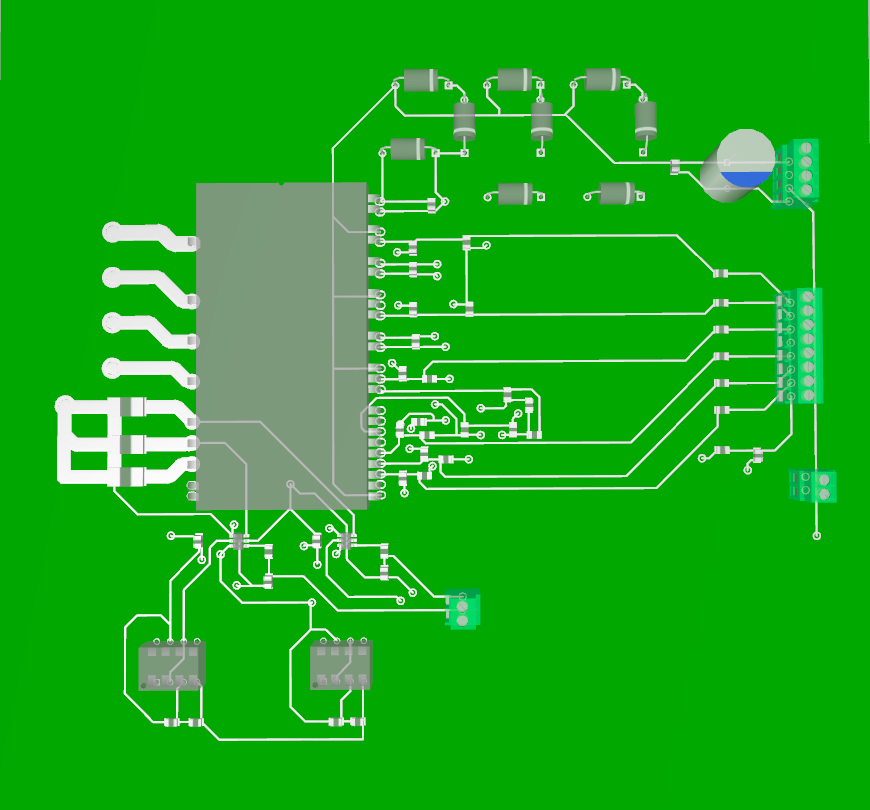
\includegraphics[width=3.5in]{sections/section4/images/PCBDesign/Ultiboard/3DTopView.png}
	\caption{3D View of PCB Layout Design in Ultiboard}
\end{figure}

This structured approach in the PCB design ensures that the board not only meets the functional requirements of the FSAM20SH60A module but also enhances reliability and performance in practical applications.

\subsection{CURRENT MEASUREMENT}

In our project, we implemented a strategy for current measurement using a shunt power resistor of 5 milli-ohms. This resistor was incorporated into two of the phase low pass filters, providing a reliable method for detecting and measuring the current flow.

Following the current detection, the signal was then directed to an IA182 operational amplifier. This component was crucial in amplifying the signal to a level suitable for further processing. The IA182 opamp was selected due to its high precision and stability, ensuring accurate amplification of the current signal.

Post amplification, the signal was fed into the Analog-to-Digital Converter (ADC) of the F28379D Launchpad. This conversion process transformed the analog current signal into a digital format, enabling the microcontroller to effectively interpret and utilize the data for further processing and control within the system. 


% Current sensing figure in multisim

\begin{figure}[H]
	\centering
	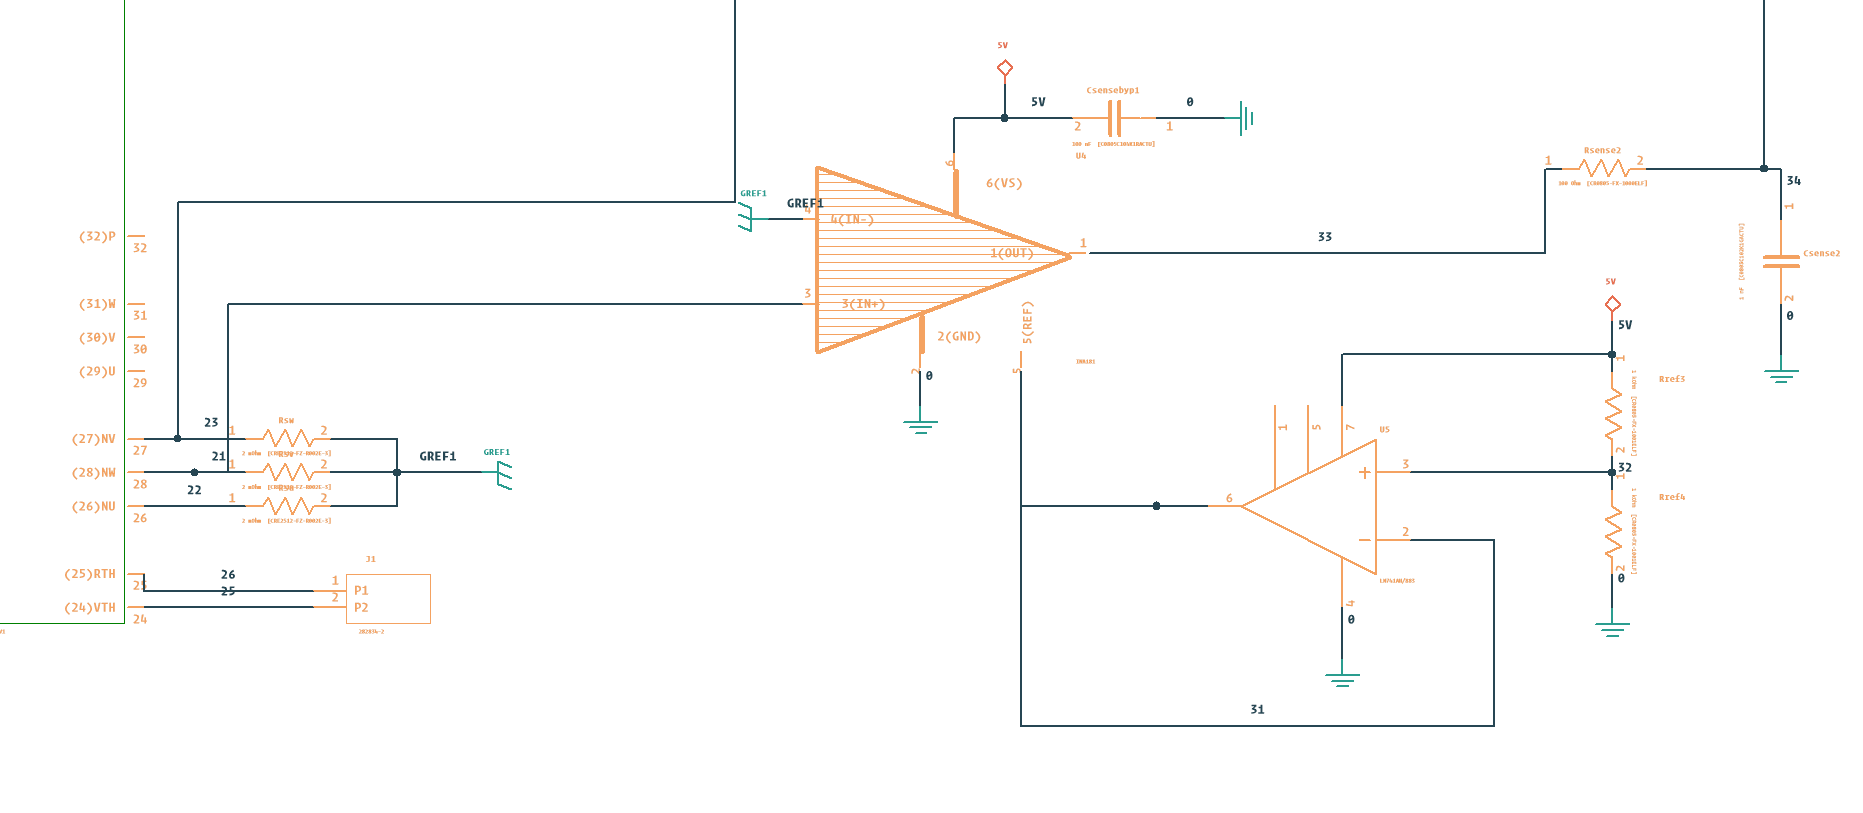
\includegraphics[width=6in]{sections/section4/images/PCBDesign/Multisim/MultisimCurrentSensing.png}
	\caption{Current Sensing Circuit in Multisim}
\end{figure}


\subsubsection{ADC Config}


\newpage